%% to produce a PDF copy, issue the following command:
%%
%%     pdflatex propositional-logic-examples.tex
%%
%% in the same directory containing the LaTeX style files:
%%
%%     prooftree.sty  and  boxproof.sty

\documentclass[11pt,leqno,fleqn]{article}

\newcommand{\tab}{\hspace*{2em}}
\usepackage{amsfonts}
\usepackage{fullpage, enumerate}
\usepackage{amsmath}
\usepackage{amssymb}
\usepackage{qtree}
\usepackage{listings}
\usepackage{graphicx}

\usepackage{tikz}
\usetikzlibrary{arrows}
\usetikzlibrary{automata}

\usepackage{graphicx} 
\usepackage{times}              % better fonts for mathematical symbols
\usepackage{bm}                 % unlike \boldmath,
                                % \bm can be used anywhere within math mode
\usepackage[scaled=0.9]{helvet} % makes text a little smaller throughout,
                                % but not the text in math mode.
%\usepackage{./tex/latex/misc/prooftree}
%\usepackage{./tex/latex/misc/boxproof}

\setlength\hoffset{-5pt}      % horizontal offset, to move text horizontally
\setlength{\textwidth}{4.5in} % try different widths
\setlength\voffset{-5pt}      % vertical offset, to move text vertically
\setlength{\textheight}{7in}  % try different heights

\newcommand{\Hide}[1]{}             % use \Hide{bla bla} to hide ``bla bla''
\newcommand{\code}[1]{\texttt{#1}}  % use \code{...} to produce ASCII chars
\newcommand{\Intro}[1]{{#1}{\textrm{i}}}
\newcommand{\Elim}[1]{{#1}{\textrm{e}}}


\newcommand{\TTT}{\bm{\mathsf{T}}}
\newcommand{\FFF}{\bm{\mathsf{F}}}

\title{CS 512, Spring 2014
       \\[1ex]
       \textbf{Assignment 8}}
\author{Shan Sikdar} 
\date{} % omit date

\begin{document}

\maketitle

\section{Problem 1}
Let $\Sigma = \{ a,b \}$. Let $L \subseteq \Sigma^*$ be a regular language.\\
Note: After taking the hints adivce and searching the internet, I used a Paper from Turku Center for Computer Science by Okhotin as a reference.
\begin{enumerate}[(a)]
\item
Since L is regular we know that there exists a NFA $\mathbf{A}$ that recognizes the regular language L.\\
w.l.o.g $\mathbf{A} = \{ S , \Sigma, \delta, Init, Final \}$\\
 (S - set of states, $\Sigma$ the alphabet, $\delta$ the transition function, Init - set if initial states, Final - set of final states).\\
 
We can extend $\bold{A}$ to $\bold{A1}$ as follows:\\
Keep S - the set of states the same.\\
Keep $\Sigma$- the alphabet the same.\\
Change $Init$ to $\{ \delta(q,w) | w \in L, q\in Init \}$\\
(Basically the new start states are the places you would go to from the original start states after you apply $w \in L$)\\
Change Final to $\{ q' \in S | \exists w \in L :\delta(q',w) \in Final \}$\\
(Basically the new set of final states will be any state you get when you apply w to an element from the original set of final states)\\
Change $\delta$ to $\delta'(q,x) = \{\delta(q,wx)|w \in L, q \in S\}$\\
So the new transition state is :\\
$\bold{A1} = \{ S, \Sigma, \{\delta(q,wx)|w \in L, q \in S\},\{ \delta(q,w) | w \in L, q\in Init \} , \{ q' \in S | \exists w \in L \delta(q',w) \in Final \} \}$\\
Since this NFA recognizes $L_{\triangleleft} \triangleq \{ u \in \Sigma^* | \text{there is a word $w \in L$ such that u $\triangleleft$ w}\}$, $L_{\triangleleft}$ is a regular language.

\item
Since L is regular we know that there exists a NFA $\mathbf{A}$ that recognizes the regular language L.\\
w.l.o.g $\mathbf{A} = \{ S , \Sigma, \delta, Init, Final \}$\\
 (S - set of states, $\Sigma$ the alphabet, $\delta$ the transition function, Init - set if initial states, Final - set of final states).\\
 
 We can extend $\bold{A}$ to $\bold{A2}$ as follows:\\
Keep S - the set of states the same.\\
Keep $\Sigma$- the alphabet the same.\\
Keep $Init$\\
Keep Final\\
Change $\delta$ to $\delta'(q,x) = \{\delta(q,x),x\}$\\
(Basically extend the transition system to have the ability to go to the state it was going to go initially, or add a self loop to that state.)\\
So essentially the NFA for Language L has been extended to have self loops in the transition system.
So the new transition state is :\\
$\bold{A2} = \{ S, \Sigma,\{\delta(q,x),x\},Init,Final \} \} $\\
Since this NFA recognizes $L_{\triangleright} \triangleq \{ u \in \Sigma^* | \text{there is a word $w \in L$ such that w $\triangleleft$ u}\}$, $L_{\triangleright}$ is a regular language.
\end{enumerate}

\newpage
\section{Problem 2}

\begin{enumerate}[(a)]
\item
$w$ contains $ab$ exactly once. \\

\begin{tikzpicture}[>=stealth',shorten >=1pt,auto,node distance=2cm]
	\node[state] (start)                {start};
	\node[state] (s0) [above right of = start] {$s_0$};
	\node[state] (s1) [below right of = start] {$s_1$};
	\node[state] (s2) [above right of = s1] {$s_2$};
	\node[state, accepting] (s3) [right of = s2] {$s_3$};
	\node[state, accepting] (s4) [right of = s3] {$s_4$};
	\path[->]	(start) edge node {$\epsilon$} (s0)
			(start) edge node {$\epsilon$} (s1)
			(s0) edge [loop above] node {$a,c$} (s0)
			(s1) edge [loop below] node {$b,c$} (s1)
			(s0) edge [bend left] node{$a$} (s2)
			(s2) edge [bend left] node{$c$} (s0)
			(s1) edge [bend left] node{$a$} (s2)
			(s2) edge [bend left] node{$c$} (s1)
			(s2) edge node{$b$} (s3)
			(s3) edge [loop above] node{$b,c$} (s3)
			(s3) edge [bend left] node{$a$} (s4)
			(s4) edge [bend left] node{$c$} (s3)
			(s4) edge [loop below] node{$a$} (s4);
\end{tikzpicture}

\item
$w$ contains $ab$ atleast once. \\

\begin{tikzpicture}[>=stealth',shorten >=1pt,auto,node distance=2cm]
	\node[state] (start)                {start};
	\node[state] (s0) [right of = start] {$s_0$};
	\node[state] (s1) [right of = s0] {$s_1$};
	\node[state, accepting] (s2) [right of = s1] {$s_2$};
	\path[->]	(start) edge node {$\epsilon$} (s0)
			(s0) edge [loop above] node {$a,b,c$} (s0)
			(s0) edge node{$a$} (s1)
			(s1) edge node{$b$} (s2)
			(s2) edge [loop above] node{$a,b,c$} (s2);
\end{tikzpicture}

\item
$w$ contains $ab$ infinitely often. \\

\begin{tikzpicture}[>=stealth',shorten >=1pt,auto,node distance=2cm]
	\node[state] (start)                {start};
	\node[state] (s0) [right of = start] {$s_0$};
	\node[state] (s1) [right of = s0] {$s_1$};
	\node[state, accepting] (s2) [right of = s1] {$s_2$};
	\path[->]	(start) edge node {$\epsilon$} (s0)
			(s0) edge [loop above] node {$b,c$} (s0)
			(s0) edge [bend left] node{$a$} (s1)
			(s1) edge [bend left] node{$c$} (s0)
			(s1) edge [loop above] node{$a$} (s1)
			(s1) edge [bend left] node{$b$} (s2)
			(s2) edge [bend left] node{$a$} (s1);
	\path[->,out=-120,in=-60]	(s2) edge node{$b,c$} (s0);
\end{tikzpicture}


\item
$w$ contains $ab$ finitely often only. In this case, we need to add accepting states that can parse all possible strings over alphabets except $ab$ to the final state of (c). The states $s_1$ and $s_2$ take care of the finitely looping part of $ab$. Hence, our new NBA will look like :\\

\begin{tikzpicture}[>=stealth',shorten >=1pt,auto,node distance=2cm]
	\node[state] (start)                {start};
	\node[state] (s0) [right of = start] {$s_0$};
	\node[state] (s1) [right of = s0] {$s_1$};
	\node[state] (s2) [right of = s1] {$s_2$};
	\node[state, accepting] (s3) [right of = s2] {$s_3$};
	\node[state, accepting] (s4) [right of = s3] {$s_4$};
	\path[->]	(start) edge node {$\epsilon$} (s0)
			(s0) edge [loop above] node {$b,c$} (s0)
			(s0) edge [bend left] node{$a$} (s1)
			(s1) edge [bend left] node{$c$} (s0)
			(s1) edge [loop above] node{$a$} (s1)
			(s1) edge [bend left] node{$b$} (s2)
			(s2) edge [bend left] node{$a$} (s1)
			(s2) edge node{$a,b,c$} (s3)
			(s3) edge [loop above] node{$b,c$} (s3)
			(s3) edge [bend left] node{$a$} (s4)
			(s4) edge [bend left] node{$c$} (s3)
			(s4) edge [loop below] node{$a$} (s4);
	\path[->,out=-120,in=-60]	(s2) edge node{$b,c$} (s0);
\end{tikzpicture}

\item
if $w$ contains infinitely often $a$s then it contains infinitely often $b$s. 
\begin{tikzpicture}[>=stealth',shorten >=1pt,auto,node distance=2cm]
	\node[state] (start)                {start};
	\node[state] (s0) [above right of = start] {$s_0$};
	\node[state, accepting] (s1) [right of = s0] {$s_1$};

	\node[state,accepting] (s2) [below right of = start] {$s_2$};
	\node[state] (s3) [right of = s2] {$s_3$};

	\path[->]	(start) edge node {$\epsilon$} (s0)
			(start) edge node {$\epsilon$} (s2)

			(s0) edge [loop above] node {$a$} (s0)
			(s0) edge [bend left] node{$b,c$} (s1)
			(s1) edge [bend left] node{$a$} (s0)
			(s1) edge [loop above] node{$b,c$} (s1)

			(s2) edge [loop above] node {$b$} (s2)
			(s2) edge [bend left] node{$a,c$} (s3)
			(s3) edge [bend left] node{$b$} (s2)
			(s3) edge [loop above] node{$a,c$} (s3);
\end{tikzpicture} \\
\end{enumerate}


\newpage
\section{Problem 3}
\begin{figure}[ht!]
\centering
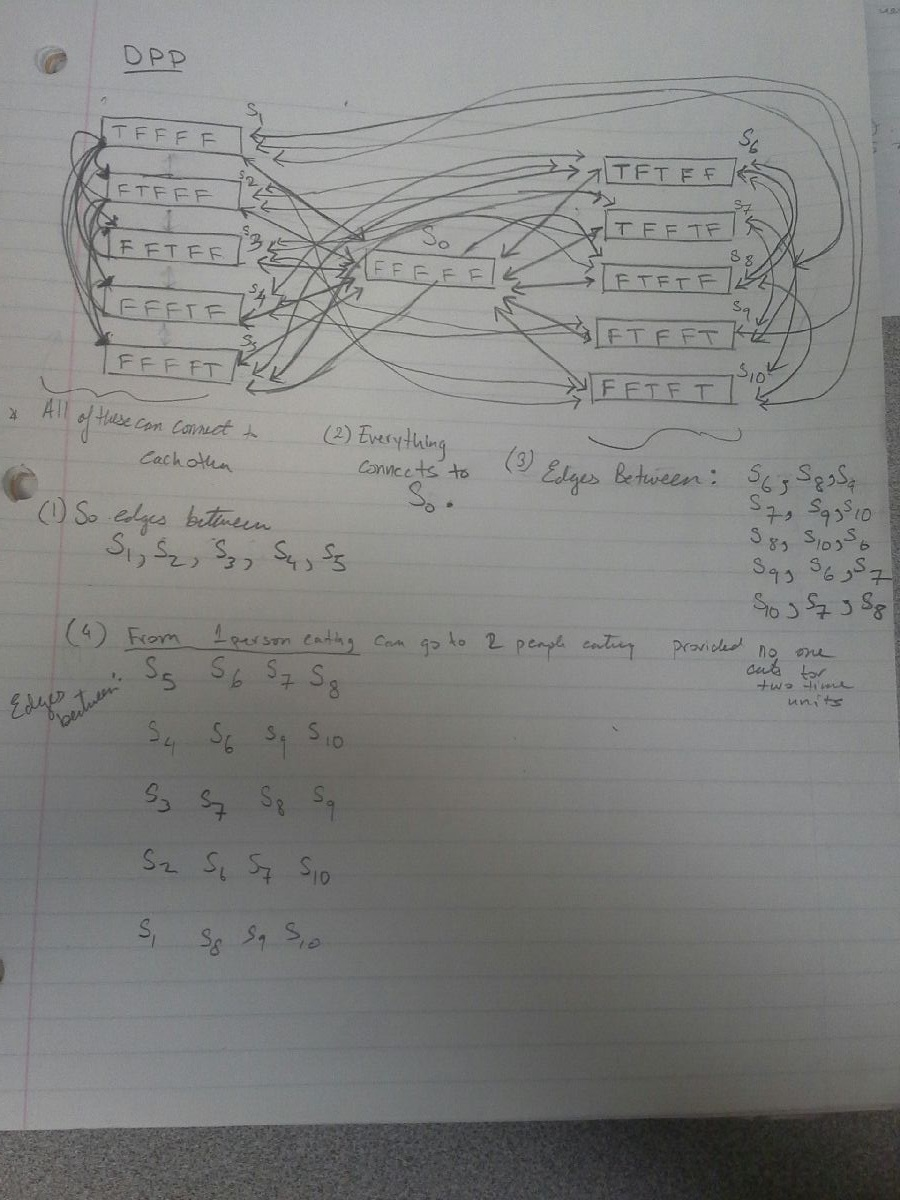
\includegraphics[width=90mm]{dpp.jpg}
\caption{DPP Model}
\label{overflow}
\end{figure}

Bonus:
\begin{enumerate}[(1)]
\item  $\mathbf{AG \neg(e_1 \land e_4)}$\\
False: look at path $s_0, s_10, ....$ the path falsifies it.
\item $\mathbf{A}(\neg(e_1 \lor e_3 \lor e_4 \lor e_5) \bold{U} e_2) $\\
False: Look at path $s_0,s_1,..$, the path falsifies the wwf.
\item True wff statisfied by the model
\item False look at path $s_0,s_8,s_0,s_4,...$ the path falsifies the wff.
\end{enumerate}


\newpage
\section{Problem 4}
The situations where deadlock occurs is a. when everyone chooses their right fork, b. when everyone chooses their left fork.
The probability of everyone choosing same side fork is $\frac{1}{2^5}$. So the probability of this happening for both these situations is $\frac{1}{32} + \frac{1}{32} = \frac{1}{16}$. So in iteration of the transition system the probability of a deadlock is $\frac{1}{16} \leq \frac{1}{10}$ So it is deadlock free with probability greater than $\frac{9}{10}$ Not only that but the probability of continuosly getting into this situation is $lim_{n \to \infty} (1/16)^n = 0$ so definiently deadlock free.
\end{document}

